\chapter{PTMcosmos}
\label{chap:ptmcosmos}



\section{Summary}



\section{Introduction}



\section{Results}


\begin{figure}[tb]
    \centering
    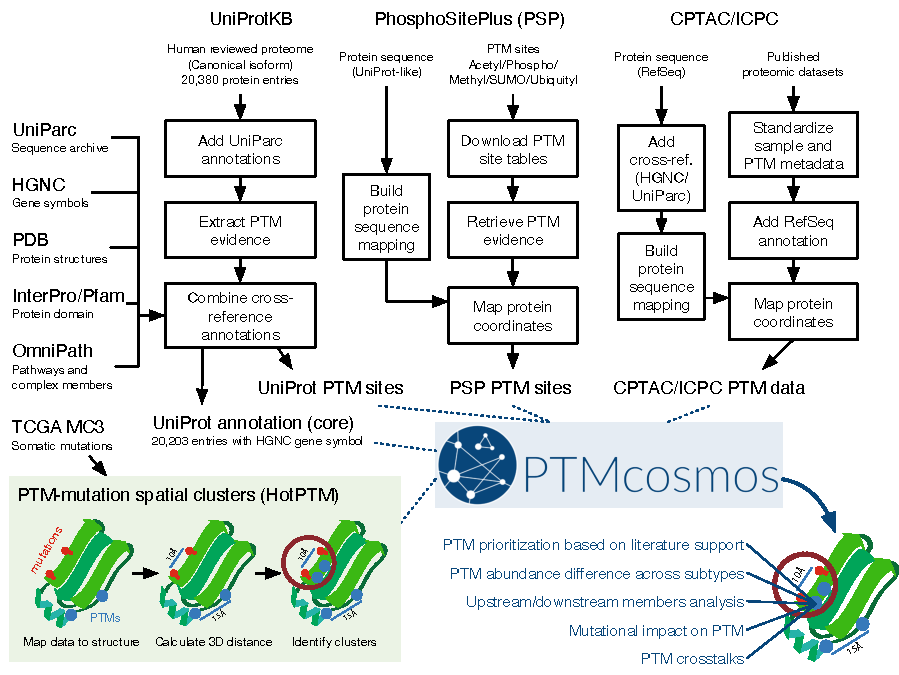
\includegraphics[width=0.9\linewidth]{figures/chap03_ptmcosmos/fig1_ptmcosmos_workflow.pdf}
    \caption[PTMcosmos overview.]{PTMcosmos overview.}
    \label{fig:ptmcosmos-workflow}
\end{figure}

\begin{figure}[tbp]
    \centering
    \phantomlabel{fig:ptmcosmos-stats-by-cancer}
    \phantomlabel{fig:ptmcosmos-stats-publications-per-ptm}
    \phantomlabel{fig:ptmcosmos-stats-publications-per-year}
    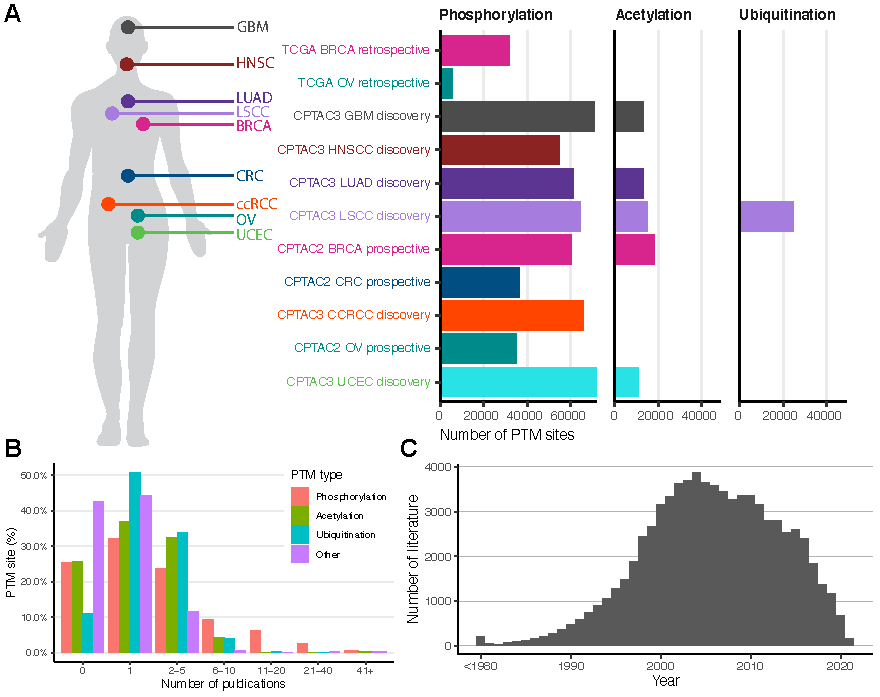
\includegraphics[width=\linewidth]{figures/chap03_ptmcosmos/fig1_ptmcosmos_stats.pdf}
    \caption[Supporting details of the mutation comparison.]{%
        Supporting details of the mutation comparison.
        \subref{fig:ptmcosmos-stats-by-cancer}
        \subref{fig:ptmcosmos-stats-publications-per-ptm}
        \subref{fig:ptmcosmos-stats-publications-per-year}
    }
    \label{fig:ptmcosmos-stats}
\end{figure}


\begin{figure}[tbp]
    \centering
    \phantomlabel{fig:ptmcosmos-map-stats-schematic}
    \phantomlabel{fig:ptmcosmos-map-stats-acetyl}
    \phantomlabel{fig:ptmcosmos-map-stats-ubiquityl}
    \phantomlabel{fig:ptmcosmos-map-stats-phospho}
    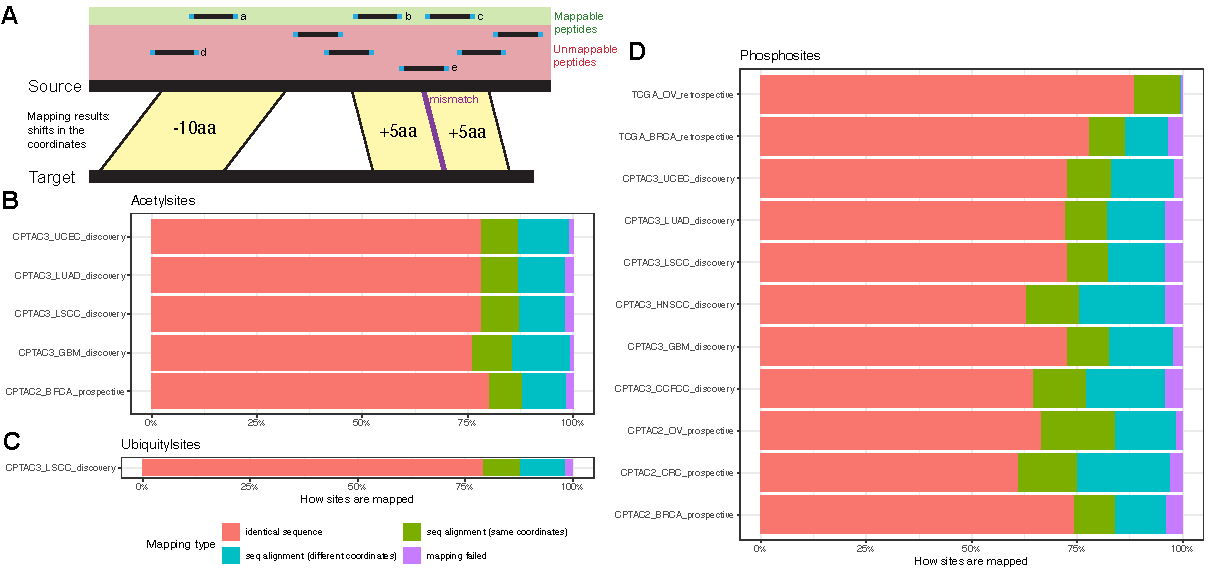
\includegraphics[width=\linewidth]{figures/chap03_ptmcosmos/figs1_mapping_stats.pdf}
    \caption[Supporting details of the peptide re-annotation and coordinate mapping.]{%
        Supporting details of the peptide re-annotation and coordinate mapping.
        \subref{fig:ptmcosmos-map-stats-schematic}
        \subref{fig:ptmcosmos-map-stats-acetyl}
        \subref{fig:ptmcosmos-map-stats-ubiquityl}
        \subref{fig:ptmcosmos-map-stats-phospho}
    }
    \label{fig:ptmcosmos-map-stats}
\end{figure}


\section{Discussion}



\section{Methods}

\subsection{CPTAC proteomic data processing}

\tref{tab:ptmcosmos-peptide-db} \url{https://github.com/ccwang002/cptac_proteome_preprocess}


\begin{table}[tbp]
    \centering
    \caption{CPTAC peptide search databases used by different disease working group.}
    \label{tab:ptmcosmos-peptide-db}
    \begin{threeparttable}[b]
    \begin{tabular}{@{}llll@{}}
    \toprule
    Phase & Cohort & Database & Notes \\
    \midrule
    \multirow{2}{*}{\begin{tabular}[c]{@{}l@{}}CPTAC2/TCGA\\ retrospective\end{tabular}}
        & BRCA  & RefSeq 20130727   & Broad Institute \\
        & OV    & RefSeq 20111201   & PNNL \\
    \midrule
    \multirow{3}{*}{\begin{tabular}[c]{@{}l@{}}CPTAC2\\ prospective\end{tabular}}
        & OV    & CDAP (Refseq 2016)    & PNNL \\
        & CRC   & RefSeq 20171003\tnote{*}  & Use RefSeq 2018 instead \\
        & BRCA  & CDAP (Refseq 2016)    & Broad Institute \\
    \midrule
    \multirow{8}{*}{\begin{tabular}[c]{@{}l@{}}CPTAC3\\ discovery\end{tabular}}
        & CCRCC & CDAP (Refseq 2018) & UMich \\
        & GBM   & CDAP (Refseq 2018) & PNNL \\
        & HNSCC & CDAP (Refseq 2018) & UMich \\
        & LUAD  & CDAP (Refseq 2018)\tnote{\textdagger} & Broad Institute \\
        & LSCC  & CDAP (Refseq 2018)\tnote{\textdagger} & Broad Institute \\
        & PBTA  & CDAP (Refseq 2018) & MS3 spectra \\
        & PDAC  & CDAP (Refseq 2018) & UMich \\
        & UCEC  & CDAP (Refseq 2018) & PNNL \\
    \bottomrule
    \end{tabular}
    \begin{tablenotes}
    \item [*] Database uses hg38 genome reference.
    \item [\textdagger] Database includes smORFs.
    \end{tablenotes}
    \end{threeparttable}
\end{table}


\subsubsection{Harmonize Coordinate}
Only considered the canonical reviewed UniProt entries 
If the identical protein sequence can be found, mapped to them directly
Otherwise, perform global protein sequence alignment
To the UniProt entry of the same gene
Create coordinate segments of consecutive matches (don't allow any amino acid mismatch)
Only mapped the site when a full peptide (plus the 1 additional flanking aa) is in the coordinate segment

